\chapter{TEST \& DESIGN}\label{cha:test}
In this chapter the methods used for testing the mobile devices for different characteristics is described. 

\section{Accelerometer \& Gyroscope}\label{sec:test:motion}
I decided to collect the data via a web-page since JavaScript can access gyroscope and accelerometer data without any permission or knowledge from the user \cite{sensor:DeviceOrientation:spec}. This only require that the device has Internet and a browser installed, no additional installations and completely cross-platform. \\
\begin{figure}[H]
  \hspace{-2cm}
  \centering
  \begin{minipage}[c]{.23\textwidth}
    \centering
    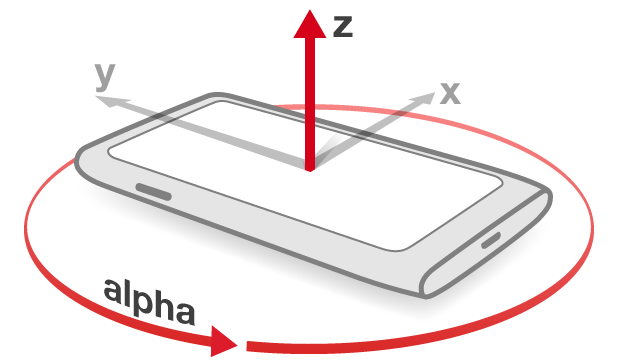
\includegraphics[scale=0.2]{img/device-alpha}
  \end{minipage}
  \hspace{1.5cm}
  \begin{minipage}[c]{.23\textwidth}
    \centering
    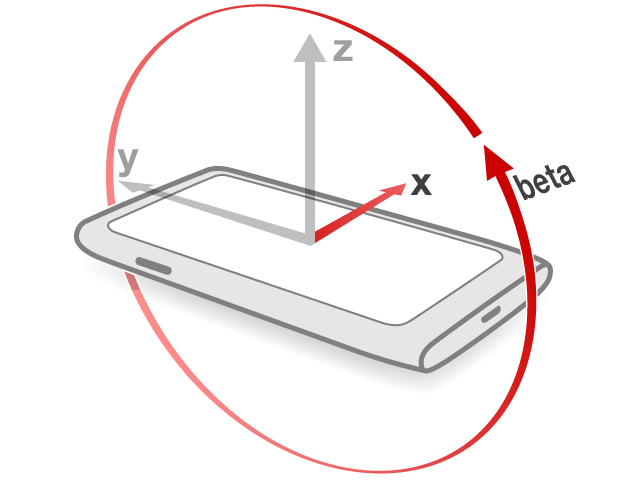
\includegraphics[scale=0.2]{img/device-beta}
  \end{minipage}
  \hspace{1.5cm}
  \begin{minipage}[c]{.23\textwidth}
    \centering
    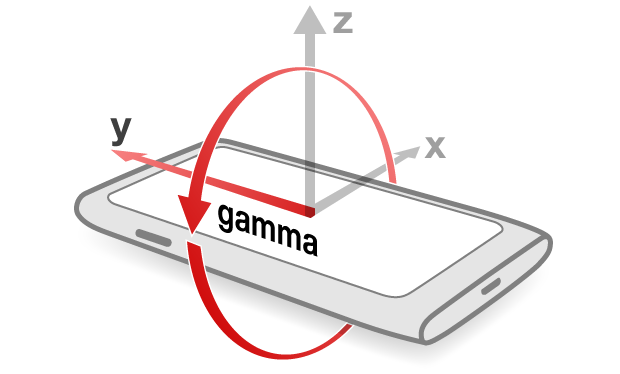
\includegraphics[scale=0.2]{img/device-gamma}
    \hspace{1cm}
  \end{minipage}
  \caption{The device axes for the JavaScript \texttt{DeviceOrientation} and \texttt{DeviceMotion}}
  \label{fig:device-axes}
\end{figure}

\subsection{Accelerometer}
For the measurements of the accelerometer a event listener is added:
\lstinputlisting{code/acc-listener.js}
In JavaScript there are two types of acceleration with and without gravity, which according to Mozilla means that \texttt{accelerationIncludingGravity} is acceleration made by the device. In context to \texttt{acceleration} not depending on influence of gravity only by the acceleration made on the device. But as I see it that acceleration is made because of gravity so it is just different point of views. Since without gravity gives no difference in scene of meters above sea level, I'll use that one. The accelerometer also comes with the nice feature of \texttt{rotationRate} which is the acceleration made from the axes in alpha, beta and gamma direction, see~\Figureref{fig:device-axes}. \cite{sensor:accIncludingGravity}\\
\\
The recording of the accelerometer is done by taking 1000 accelerator-data samples during a few seconds and saved in a CSV for analyzing. Since there are six different measurements that gives a 6-by-1000 matrix for each device as a base for accelerometer characteristics. When gather all devices together in a six-dimension space that includes clusters of all device samples. For knowing the distance between this measurements MATLAB is used. To know the difference between measurements from the devices, the Euclidean norm value is calculated. Norm is a function that gives a size to a vector.  The norm for one vector is calculated like;
$$\|\boldsymbol{x}\| := \sqrt{x_1^2 + \cdots + x_n^2}.$$
This is done for each of the six measurement-vectors. And then summed up like
$$(abs(V_x)^6 + abs(V_y)^6 + abs(V_z)^6 + abs(V_alpha)^6 + abs(V_beta)^6 + abs(V_gamma)^6)^(1/6)$$
In MATLAB this looks like:
\begin{lstlisting}[language=Matlab]
 motion = importdata(motion.csv);
 norm = norm(motions.data, 6);
\end{lstlisting}
A nearest neighbor algorithm called \texttt{pdist2} that calculates the pairwise euclidean distance between two sets of observations;
\begin{lstlisting} 
 D = pdist2(X,Y,`euclidean'); 
 
\end{lstlisting}
Where X us an x-by-n matrix and Y is an y-by-n matrix. 

\subsection{Gyroscope}
For the measurements of the gyroscope another event listener is added:
\lstinputlisting{code/gyro-listener.js}
The \texttt{DeviceOrientation} is using the same axes as the accelerometer but the gyroscope is measuring how much the device is rotating along the \texttt{alpha, beta} and \texttt{gamma} axes in degrees (\Figureref{fig:device-axes}). The \texttt{alpha} is between 0 and 360 degrees, \texttt{beta} -180 to 180 degrees and \texttt{gamma} -90 to 90 degrees. \citet{sensor:DeviceOrientation:spec}

\section{Sound}\label{sec:test:sound}
For distinguish these error characteristics for fingerprinting \cite{sensor:micSpek} used an application in the mobile device. The application played a sound from the speakers, recorded by the microphone that send its output back to the application. This were applied in a quiet environment due to minimizing signal noise.

\section{Camera}\label{sec:test:camera}
e basic algorithm for linking a camera to an image is quite simple. First we calculate the camera reference patterns (essentially an approximation to f), then we look for a correlation between each of these patterns and the noise of an image. e easiest way to calculate an approximation to the camera reference pattern is to average multiple images. To speed up this process we can first remove the scene content using a denoising filter and then average the noise residuals instead. Based on experimentation, Lukáš et al. found a wavelet-based filter gave the best results as it removed the most traces of the scene. e technique also works better with uniformly lit images with no features so we only get noise from the sensor. e larger the number of images we average over, the more we suppress random noise
and the impact of any scene data; a minimum of 50 images is recommended. Once we have established this reference pattern, we can see if there is a correlation with the noise of a particular image. To find the noise, we employ the same trick as before: Use the denoising filter to approximate the noise-free image and subtract this (on a pixel-wise basis) from the original, leaving only the noise residual. We then find the correlation between this noise n and a particular reference pattern r using the standard formula:
By experimentally determining the distribution of this correlation for images taken with a camera and images not taken with that camera we can find a threshold for acceptance and estimate the false rejection rate, subject to an upper bound on
the false acceptance rate. \cite[p.2]{sensor:camera:DCIdent}

\section{Gyroscope Accelerometer}\label{sec:test:gyro}
TIPS TESTMETOD: In this section we describe a technique known as Allan Variance, which can be used to detect and determine the properties of such processes. We then apply this technique to the accelerometer and gyroscope signals emitted from an Xsens Mtx device \cite{sensor:inertialNav} \\
ACC KANSKE SKA ANVÄNDA DENNA: \cite{sensor:micSpek} \\

Testa först:
Hämta data från acc o gyro när mobilen ligger stilla och data från vibration.

\section{Radio signal}\label{sec:test:rff}
PARADIS ?
